\input{"C:/Users/spileggi/Google Drive/STAT 330/Lectures/SlideStyle.tex"}



\title[Lecture 10]{How the DATA step works, PROC SGPLOT}
\author[Pileggi]{Shannon Pileggi}

\institute[STAT 330]{STAT 330}

\date{}


\begin{document}

\begin{frame}
\titlepage
\end{frame}

\begin{frame}
\frametitle{OUTLINE\qquad\qquad\qquad} \tableofcontents[hideallsubsections]
\end{frame}


%===========================================================================================================================
\section[How the DATA step works]{How the DATA step works}
%===========================================================================================================================
\subsection{}
%\begin{frame}
%\tableofcontents[currentsection, hideallsubsections]
%\end{frame}

\begin{frame}
\ft{How DATA steps work}
The purpose of the DATA step is \emph{read}, \emph{modify}, or \emph{create} data.  How does it work?  SAS executes the DATA step line by line \ttb{and} observation by observation.
\vskip10pt
SAS has a built in loop!
\bi
\item all lines of the data step are executed on observation 1
\item all lines of the data step are executed on observation 2
\item all lines of the data step are executed on observation 3
\item etc.
\ei
\end{frame}

\begin{frame}[fragile]
\ft{Example data}
\bmp{0.80\textwidth}
\footnotesize
\begin{code}{.0}
DATA class;
  INPUT name \$ GPA dob MMDDYY10. salary COMMA8.;
  DATALINES;
  Bill  3.4  10/13/1995 \$18,000
  Susan 2.7  6/24/1993  \$535,000
  ;
RUN;
\end{code}
\emp
\end{frame}

\begin{frame}[label=action]
\ft{DATA step actions}
When you submit a DATA step, it goes through the
\vskip10pt
\begin{enumerate}
    \item Compile phase \hyperlink{compilephases}{\beamerreturnbutton{Jump to it}}
    \item Execution phase \hyperlink{execution}{\beamerreturnbutton{Jump to it}}
\end{enumerate}
\vskip10pt
\url{http://support.sas.com/documentation/cdl/en/basess/58133/HTML/default/viewer.htm#a001290590.htm}
\end{frame}

\begin{frame}[label=compilephases]
\ft{Compile phase}
During the compile phase, SAS compiles statements, checks syntax, and creates:
\begin{enumerate}
    \item  descriptor information \hyperlink{descriptor}{\beamerreturnbutton{More info}}
    \item  an input buffer \hyperlink{input}{\beamerreturnbutton{More info}}
    \item  a Program Data Vector (PDV) \hyperlink{pdvC}{\beamerreturnbutton{More info}}
\end{enumerate}
\begin{flushright}
\hyperlink{action}{\beamerreturnbutton{Back to DATA step actions}}
\end{flushright}
\end{frame}

\begin{frame}[label=descriptor]
\ft{Descriptor information}
\bi
\item Descriptor information is information that SAS creates and maintains about each SAS data set
\item This includes data set attributes and variable attributes
\item for example, the date data set was created, names and types of variables.
\item To see some descriptor information, submit
\item[] \fbox{\ttt{PROC CONTENTS DATA = class;  RUN;}}
\ei
\begin{flushright}
\hyperlink{compilephases}{\beamerreturnbutton{Back to compile phases}}
\end{flushright}
\end{frame}



\begin{frame}[label=input]
\ft{Input buffer}
\bi
\item logical area in memory into which SAS reads each record of raw data when executing an input statement
\item only used for reading ``raw'' data (not a SAS data set)
\item[]
\ei
\resizebox{1.0\textwidth}{!}{
\begin{tabular}{|l|l|l|l|l|l|l|l|l|l|l|l|l|l|l|l|l|l|l|l|l|l|l|l|l|l|l|l|l|l|}
\hline
0	&	1	&	2	&	3	&	4	&	5	&	6	&	7	&	8	&	9	&	0	&	1	&	2	&	3	&	4	&	5	&	6	&	7	&	8	&	9	&	0	&	1	&	2	&	3	&	4	&	5	&	6	&	7	&	8	&	9	\\
\hline
B	&	i	&	l	&	l	&		&	3	&	.	&	4	&		&	1	&	0	&	/	&	1	&	3	&	/	&	1	&	9	&	9	&	8	&		&	\$	&	1	&	8	&	,	&	0	&	0	&	0	&		&		&		\\
\hline
\end{tabular}}\\
\vskip10pt
\begin{flushright}
\hyperlink{compilephases}{\beamerreturnbutton{Back to compile phases}}
\end{flushright}
\end{frame}




\begin{frame}[label=pdvC]
\ft{Program Data Vector - Compile phase}
\bi
\item The PDV is as a virtual row of the SAS data set.
\item The PDV begins with all missing entries.
\item Two temporary variables are created during the processing of every data step as part of the PDV.
\begin{enumerate}
\item \ttb{\ttt{\_N\_}} is the DATA step iteration counter
\item \ttb{\ttt{\textunderscore ERROR\textunderscore}} indicates the data error status
    \bi
    \item[] 0 =  no data error on that record
    \item[] 1 = at least one data error on that record
    \ei
\end{enumerate}
\ei
\begin{center}
\begin{tabular}{|l|l|l|l|l|l|}
\hline
\ttb{\ttt{\textunderscore N\textunderscore}} & \ttb{\ttt{\textunderscore ERROR\textunderscore}} & \ttb{\ttt{name}} & \ttb{\ttt{GPA}} & \ttb{\ttt{dob}} & \ttb{\ttt{salary}} \\
\hline
1 & 0 &  & . & . & .  \\
\hline
\end{tabular}
\end{center}
\begin{flushright}
\hyperlink{pdvE}{\beamerreturnbutton{PDV in execution phase}}
\hyperlink{compilephases}{\beamerreturnbutton{Back to compile phases}}
\end{flushright}
\end{frame}

\begin{frame}[label=execution]
\ft{Execution phase}
\bi
    \item counts iterations of the DATA step (at the top)
    \item sets all values in PDV to missing
    \item reads input record (if relevant)
    \item executes additional manipulation/computation \hyperlink{pdvE}{\beamerreturnbutton{Program Data Vector in the Execution Phase}}
    \item writes record to output data set
\ei
\begin{flushright}
\hyperlink{action}{\beamerreturnbutton{Back to DATA step actions}}
\end{flushright}
\end{frame}


\begin{frame}[label=pdvE]
\ft{Program Data Vector - Execution phase}
\bi
\item PDV entries are specified one column at a time.
\item the PDV copies its contents into the SAS data set matrix filling a complete row (observation).
\item the PDV empties and the process begins again.
\item[]
\ei
\begin{center}
\begin{tabular}{|l|l|l|l|l|l|}
\hline
\ttb{\ttt{\textunderscore N\textunderscore}} & \ttb{\ttt{\textunderscore ERROR\textunderscore}} & \ttb{\ttt{name}} & \ttb{\ttt{GPA}} & \ttb{\ttt{dob}} & \ttb{\ttt{salary}} \\
\hline
1 & 0 & Bill & 3.4 & 13069 & 18000  \\
\hline
\end{tabular}
\end{center}
\begin{flushright}
\hyperlink{pdvC}{\beamerreturnbutton{PDV in compile phase}}
\hyperlink{action}{\beamerreturnbutton{Back to DATA step actions}}
\end{flushright}
\end{frame}


\begin{frame}
\ft{Running the SAS DATA step}
\bmp{0.1\textwidth}
\hspace{0.1in}
\emp
\bmp{0.9\textwidth}
\begin{itemize}
\footnotesize{
\item[Compile]  SAS examines program for syntax errors and creates PDV with values set to missing
\item[Execution 1]SAS reads Bill's record from the input buffer to the PDV one variable at a time
\item[Execution 2]SAS calculates the day of the week Bill was born on and stores it in the PDV
\item[Execution 3]SAS writes values in the PDV to the first observation in the \ttt{class} data set
\item[Execution 4]SAS returns to the the top of the DATA step and resets values in the PDV to missing, \ttt{\textunderscore N\textunderscore} changes to 2
\item[Execution 5]SAS reads Susan's record from the input buffer to the PDV one variable at a time
\item[Execution 6]SAS calculates the day of the week Susan was born on and stores it in the PDV
\item[Execution 7]SAS writes values in the PDV to the second observation in the \ttt{class} data set
\item[Cycle Ends]\textcolor{white}{p}}
\end{itemize}
\emp
\end{frame}

\begin{frame}
\ft{Discussion}
\begin{clicker}{Suppose you run a program that causes three DATA step errors where the last iteration ends on an error. At the end of the data step, what is the value of the automatic variable
\ttt{\textunderscore ERROR\textunderscore}?}
0   \hspace{0.2in} 1  \hspace{0.2in} 2 \hspace{0.2in}  3
\end{clicker}
\end{frame}

\begin{frame}[fragile]
\ft{Example error in PDV}
\bmp{1.0\textwidth}
\footnotesize
\begin{code}{.0}
DATA class;
  INPUT name \$ GPA dob MMDDYY10. salary COMMA8.;
  DATALINES;
  Bill  3.4 10/13/1995  \$18,000
  Susan 2.7 \textcolor{OrangeRed}{06/24/199}  \$535,000
  ;
RUN;
\end{code}
\emp 
\vspace{2ex}
\bmp{1.0\textwidth}
\footnotesize
\begin{craw}{.0}{SAS log}
NOTE: Invalid data for dob in line 106 13-22.
RULE:      ----+----1----+----2----+----3----+----4----+----5----+----6----+----7----+----8----+-
106          Susan 2.7 06/24/199  \$535,000
name=Susan GPA=2.7 dob=. salary=53500 _ERROR_=1 _N_=2
\end{craw}
\emp
\end{frame}

\begin{frame}[fragile]
\ft{Discussion}
\begin{clicker}{Which output will this code generate?}
\end{clicker}
\bmp{0.4\textwidth}
\footnotesize
\begin{code}{.0}
DATA one;
  \textcolor{OrangeRed}{OUTPUT;}
  DO i = 1 to 4;
	 x = i**3;
	 \textcolor{OrangeRed}{OUTPUT;}
  END;
  \textcolor{OrangeRed}{OUTPUT;}
RUN;
PROC PRINT DATA = one;
RUN;
\end{code}
\emp
\bmp{0.05\textwidth}
\hspace{0.05in}
\emp
\bmp{0.2\textwidth}
Ouptut 1 \\
\begin{tabular}{|ll|}
\hline
\ttt{i} & \ttt{x} \\
. & .\\
1 & 1 \\
2 & 8 \\
3 & 27 \\
4 & 64 \\
5 & 64 \\
\hline
\end{tabular}
\emp
\bmp{0.2\textwidth}
Ouptut 2 \\
\begin{tabular}{|ll|}
\hline
\ttt{i} & \ttt{x} \\
1 & 1 \\
2 & 8 \\
3 & 27 \\
4 & 64 \\
\hline
\end{tabular}
\vspace*{0.35in}
\emp
\bmp{0.2\textwidth}
Ouptut 3 \\
\begin{tabular}{|ll|}
\hline
\ttt{i} & \ttt{x} \\
1 & 1 \\
2 & 8 \\
3 & 27 \\
4 & 64 \\
4 & 64 \\
\hline
\end{tabular}
\vspace*{0.15in}
\emp

\end{frame}

%\begin{frame}
%\ft{Discussion}
%\begin{clicker}{The program data vector is only used during the compile phase of the DATA step.}
%\begin{enumerate}
%    \item True
%    \item False
%\end{enumerate}
%\end{clicker}
%\end{frame}



%===========================================================================================================================
\section[PROC SGPLOT]{PROC SGPLOT}
%===========================================================================================================================
\subsection{}
\begin{frame}
\tableofcontents[currentsection, hideallsubsections]
\end{frame}

\begin{frame}
\ft{PROC SGPLOT}
PROC SGPLOT is a stand alone procedure for making graphics.
\bi
\item \ttt{HBAR/VBAR} = bar chart
\item \ttt{HISTOGRAM} = histogram
\item \ttt{VBOX/HBOX} = box plot
\item \ttt{SCATTER} = scatter plot
\item \ttt{SERIES} = time series plots
\ei
\end{frame}


\begin{frame}[fragile]
\ft{Getting started}
The \ttt{O2012.sas7bdat} data set contains information on athletes that won medals in the 2012 olympics, including the country that they represented, the sport they competed in, and the total number of medals earned.
\vskip10pt
\oyo
\begin{enumerate}
    \item Write a libname statement to access the \ttt{O2012} data set.
    \item Examine the contents of the \ttt{O2012} data set.  How many observations are there?
    \item Explore the data set.
\end{enumerate}
\end{frame}

\begin{frame}
\ft{Review question}
\begin{clicker}{Which code can be used to obtain the number of athletes who won medals in \ttt{Swimming} for the participating countries?}
\begin{enumerate}
\item \ttt{proc freq data=flash.o2012; tables country;
\item[] where sport="Swimming"; run;}
\item \ttt{proc means data=flash.o2012; var country;
\item[] where sport="Swimming"; run;}
\item \ttt{proc freq data=flash.o2012; tables country;
\item[] if sport="Swimming"; run;}
\item \ttt{proc freq data=flash.o2012; tables country;
\item[] class sport="Swimming"; run;}
\item \ttt{proc univariate data=flash.o2012; tables sport;
\item[] class country; run;}
\end{enumerate}
\end{clicker}
\end{frame}


\begin{frame}[fragile]
\ft{Bar plot in PROC FREQ}
\bmp{0.65\textwidth}
\footnotesize
\begin{code}{.0}
PROC FREQ DATA = flash.o2012;
   TABLES country / PLOTS = freqplot;
   WHERE sport = "Swimming";
RUN;
\end{code}
\emp
\vspace{1ex}
\bmp{0.6\textwidth}
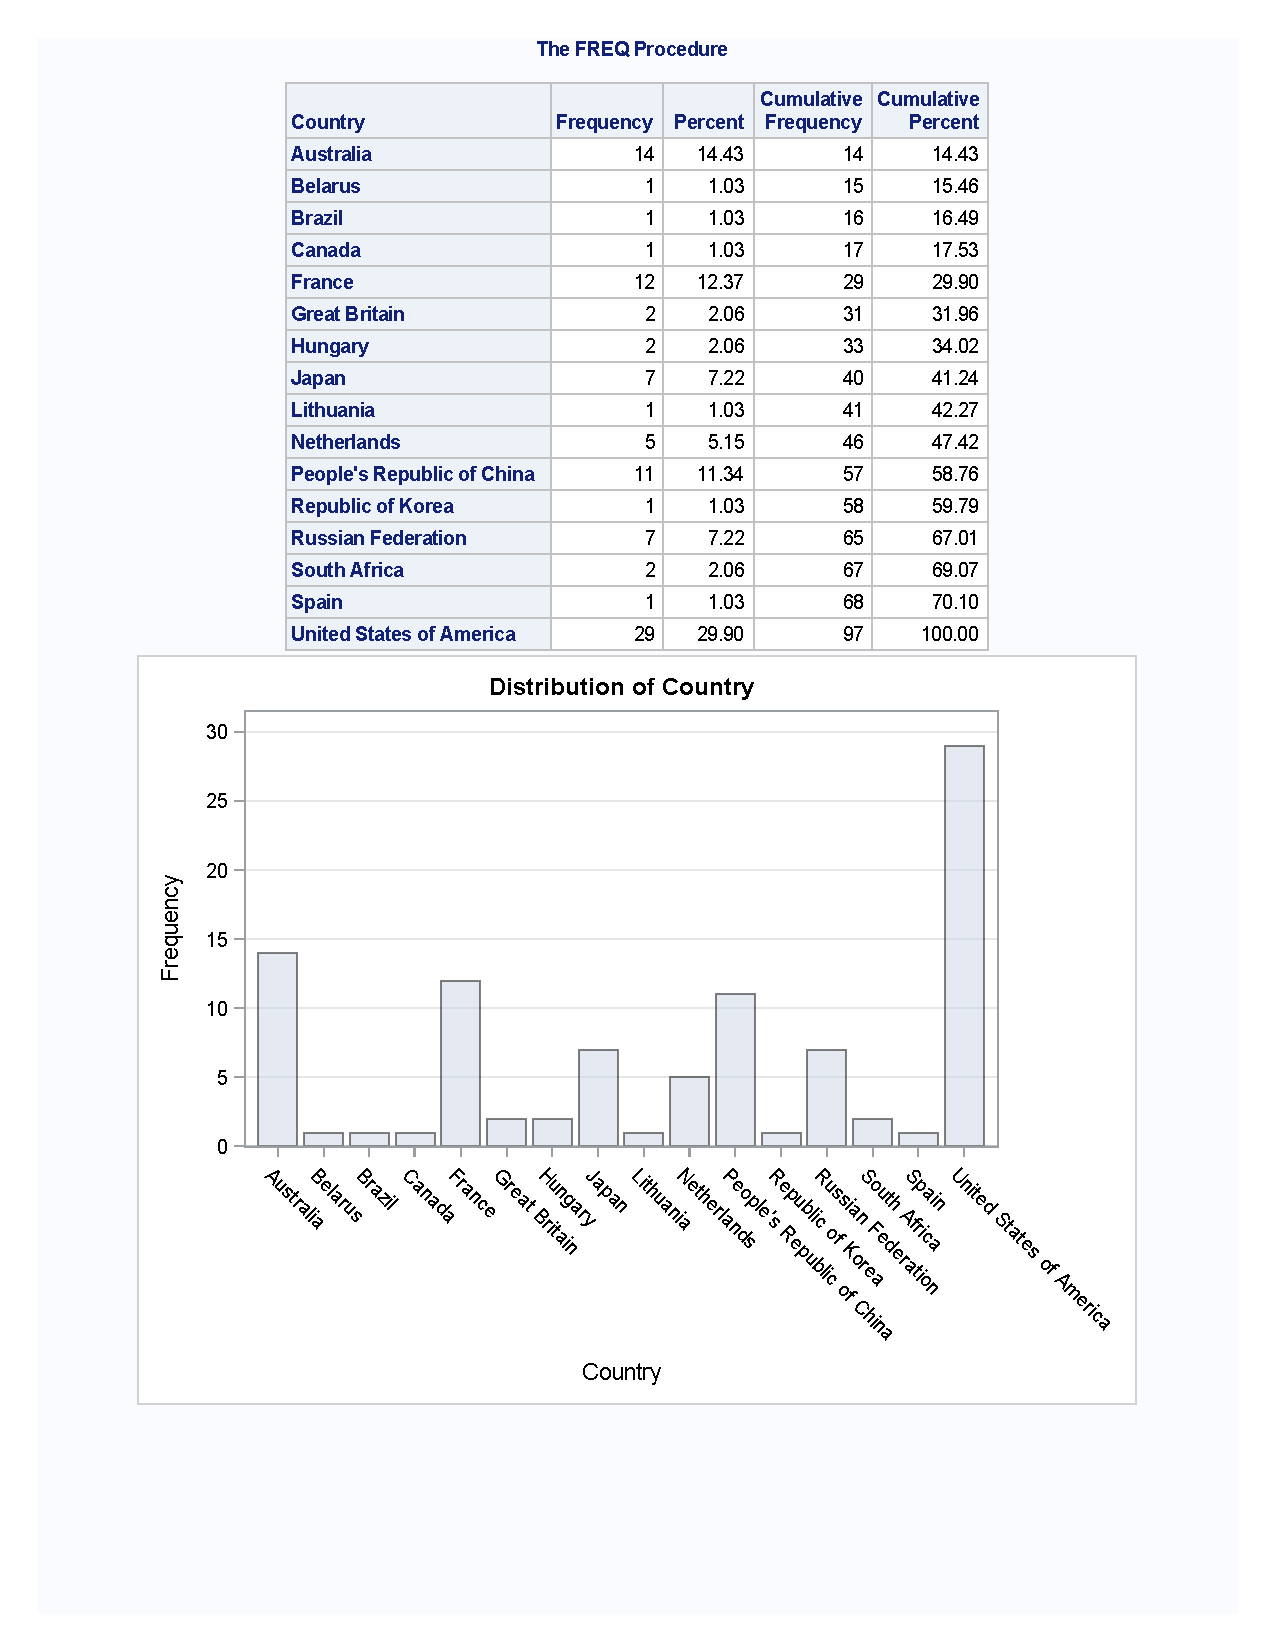
\includegraphics[trim=1.5cm 2cm 1.5cm 11.5cm,clip,width=1.0\textwidth]{L10_procfreqbarplot.pdf}
\emp
\end{frame}


\begin{frame}[fragile]
\ft{Bar plot in PROC SGPLOT}
\bmp{0.65\textwidth}
\footnotesize
\begin{code}{.0}
PROC SGPLOT DATA = flash.o2012;
	WHERE sport="Swimming";
	VBAR country ;
RUN;
\end{code}
\emp
\vspace{1ex}
\bmp{0.6\textwidth}
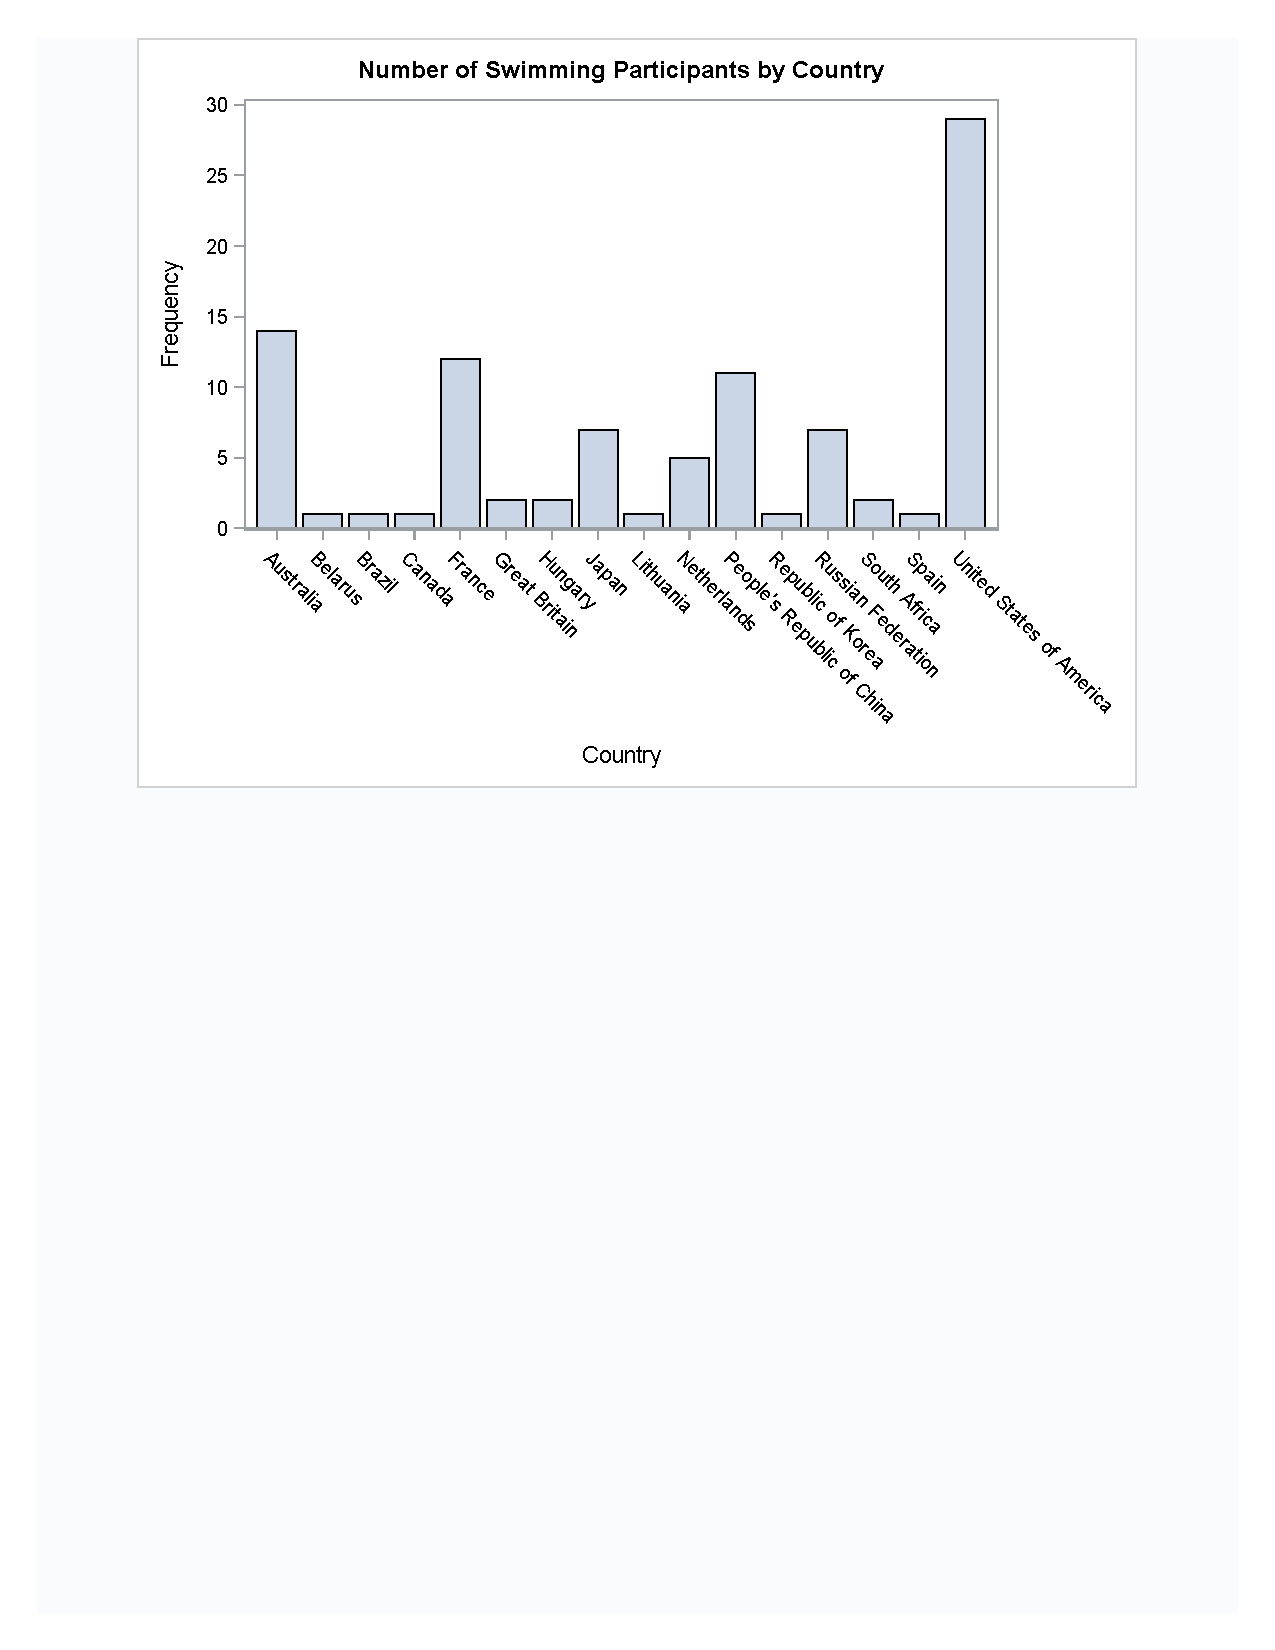
\includegraphics[trim=1.5cm 15cm 1.5cm 0cm,clip,width=1.0\textwidth]{L10_procsgplotbarplot}
\emp
\end{frame}

\begin{frame}[fragile]
\ft{Bar plot, weighted count}
\bmp{1.00\textwidth}
\footnotesize
\begin{code}{.0}
PROC SGPLOT DATA = flash.o2012 ;
	where sport = "Swimming";
	VBAR country / \textcolor{OrangeRed}{RESPONSE = total} ;
RUN ;
\end{code}
\emp
\vspace{1ex}
\bmp{0.6\textwidth}
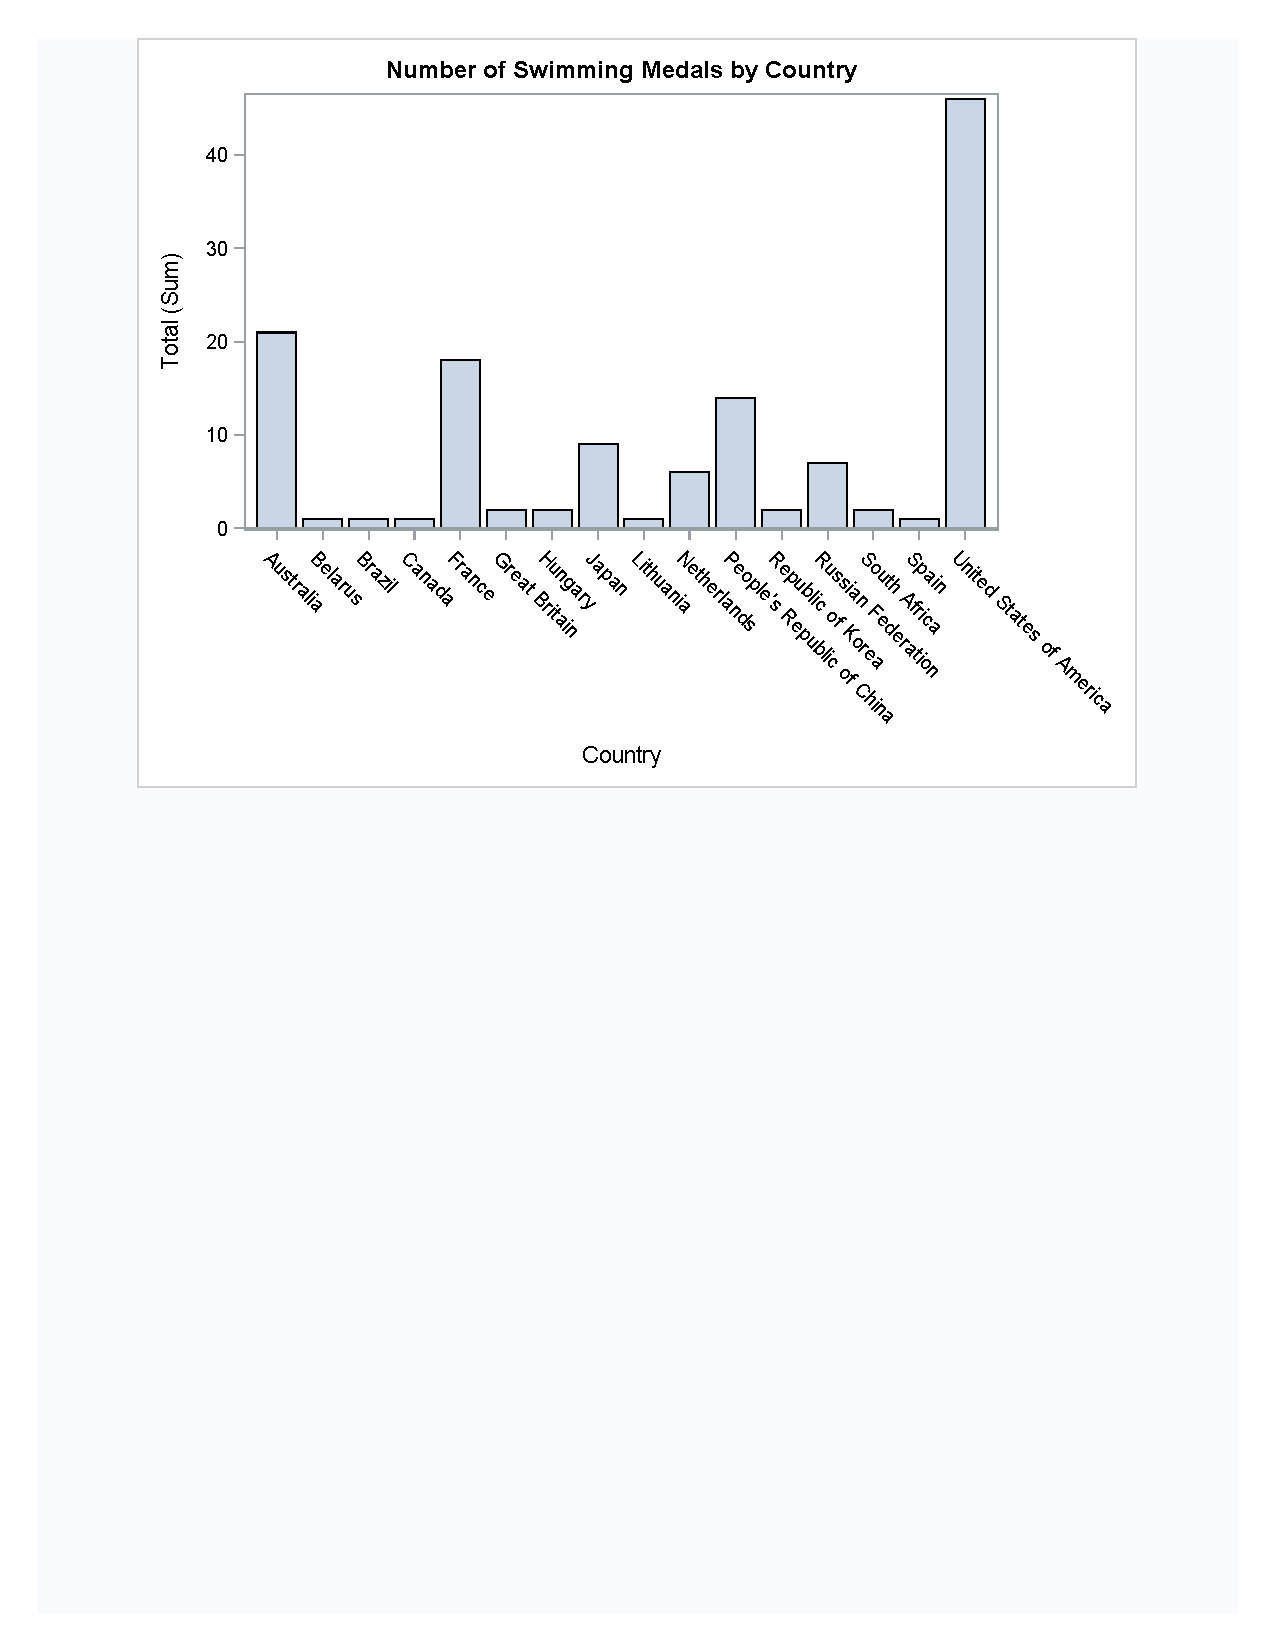
\includegraphics[trim=1.5cm 15cm 1.5cm 0cm,clip,width=1.0\textwidth]{L10_procsgplotbarplotresponse}
\emp
\end{frame}


\begin{frame}[fragile]
\ft{Bar plot, stacked}
\bmp{1.00\textwidth}
\footnotesize
\begin{code}{.0}
PROC SGPLOT DATA = flash.o2012;
	WHERE sport="Swimming" or sport="Rowing";
	VBAR country / \textcolor{OrangeRed}{GROUP = sport} RESPONSE = total ;
RUN;
\end{code}
\emp
\vspace{1ex}
\bmp{0.6\textwidth}
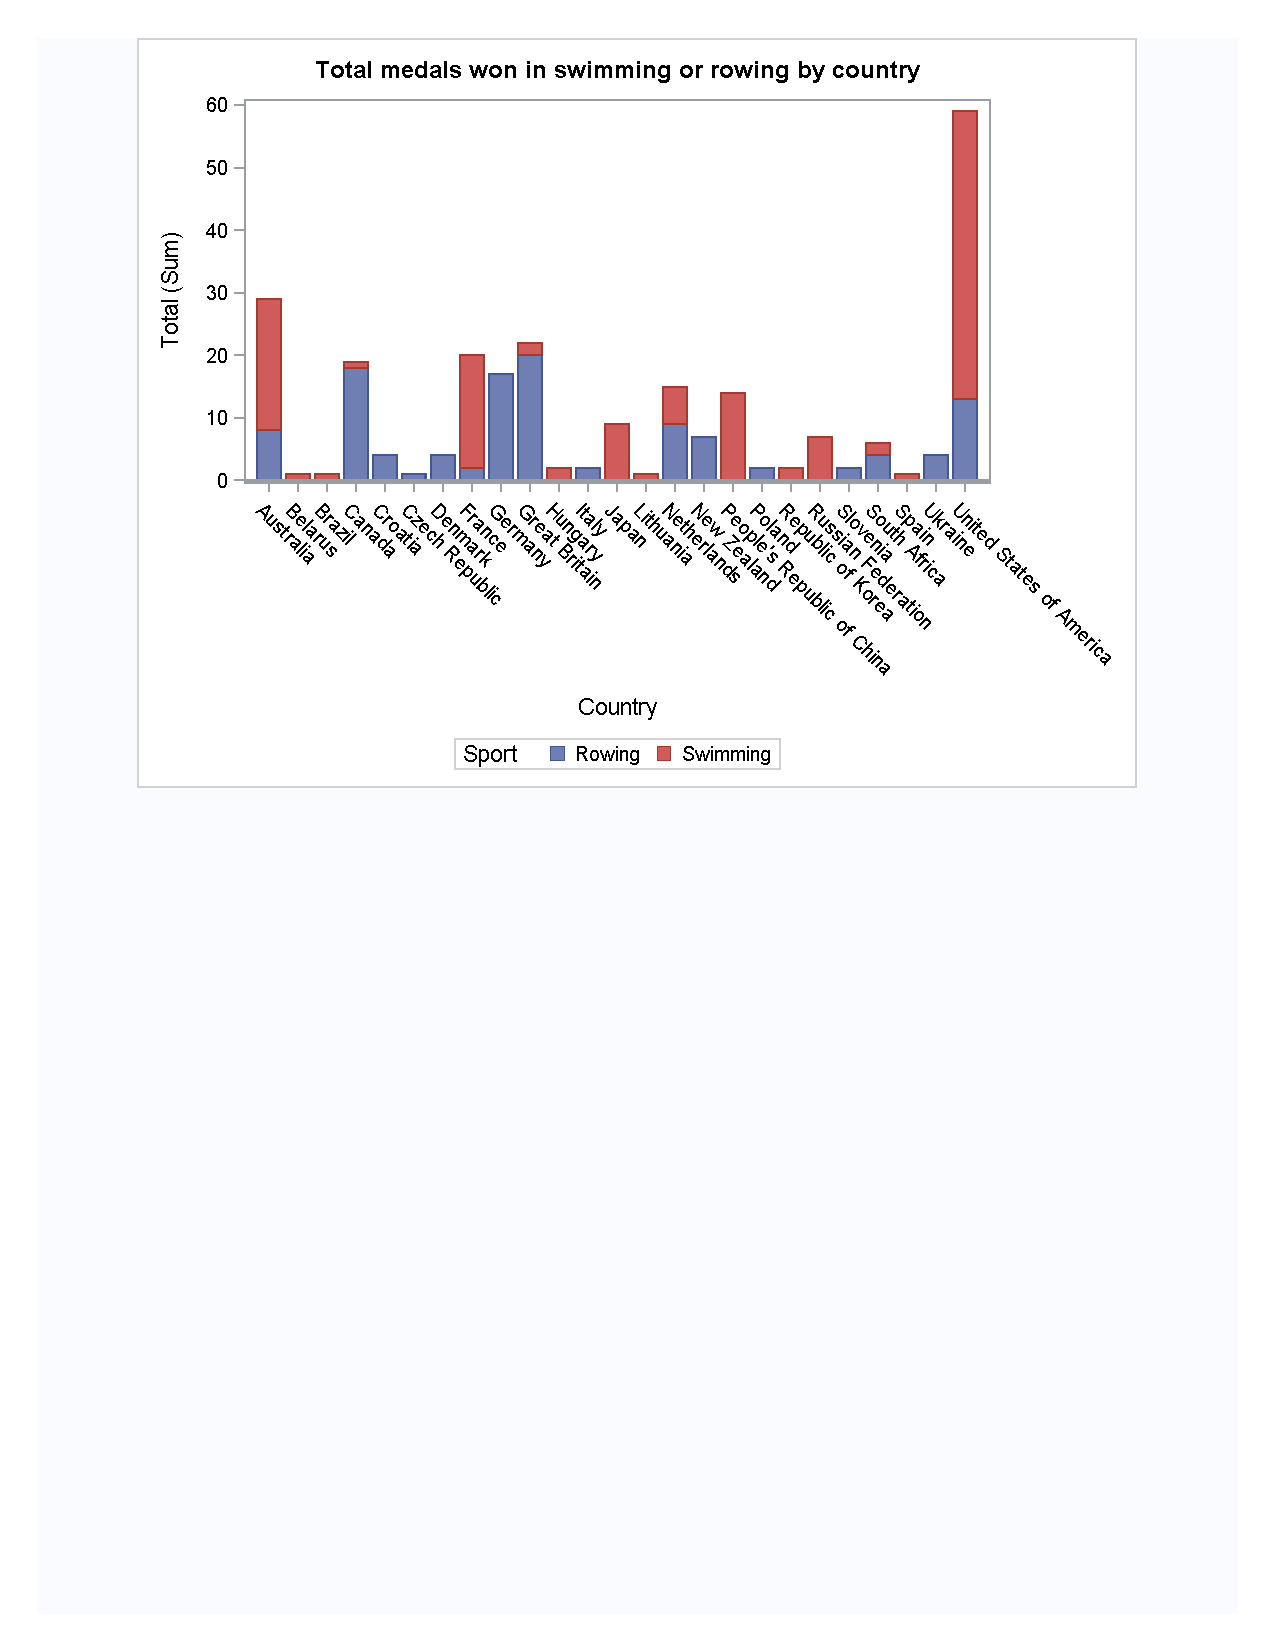
\includegraphics[trim=1.5cm 15cm 1.5cm 0cm,clip,width=1.0\textwidth]{L10_procsgplotbarplotresponsestacked}
\emp
\end{frame}

\begin{frame}[fragile]
\ft{Bar plot, add vertical lines}
\bmp{1.00\textwidth}
\footnotesize
\begin{code}{.0}
PROC SGPLOT DATA = flash.o2012;
   WHERE sport="Swimming" ;
   VBAR country / RESPONSE = total ;
   \textcolor{OrangeRed}{VLINE} country / RESPONSE = gold ;
   \textcolor{OrangeRed}{VLINE} country / RESPONSE = silver ;
   \textcolor{OrangeRed}{VLINE} country / RESPONSE = bronze ;
RUN ;
\end{code}
\emp
\vspace{1ex}
\bmp{0.6\textwidth}
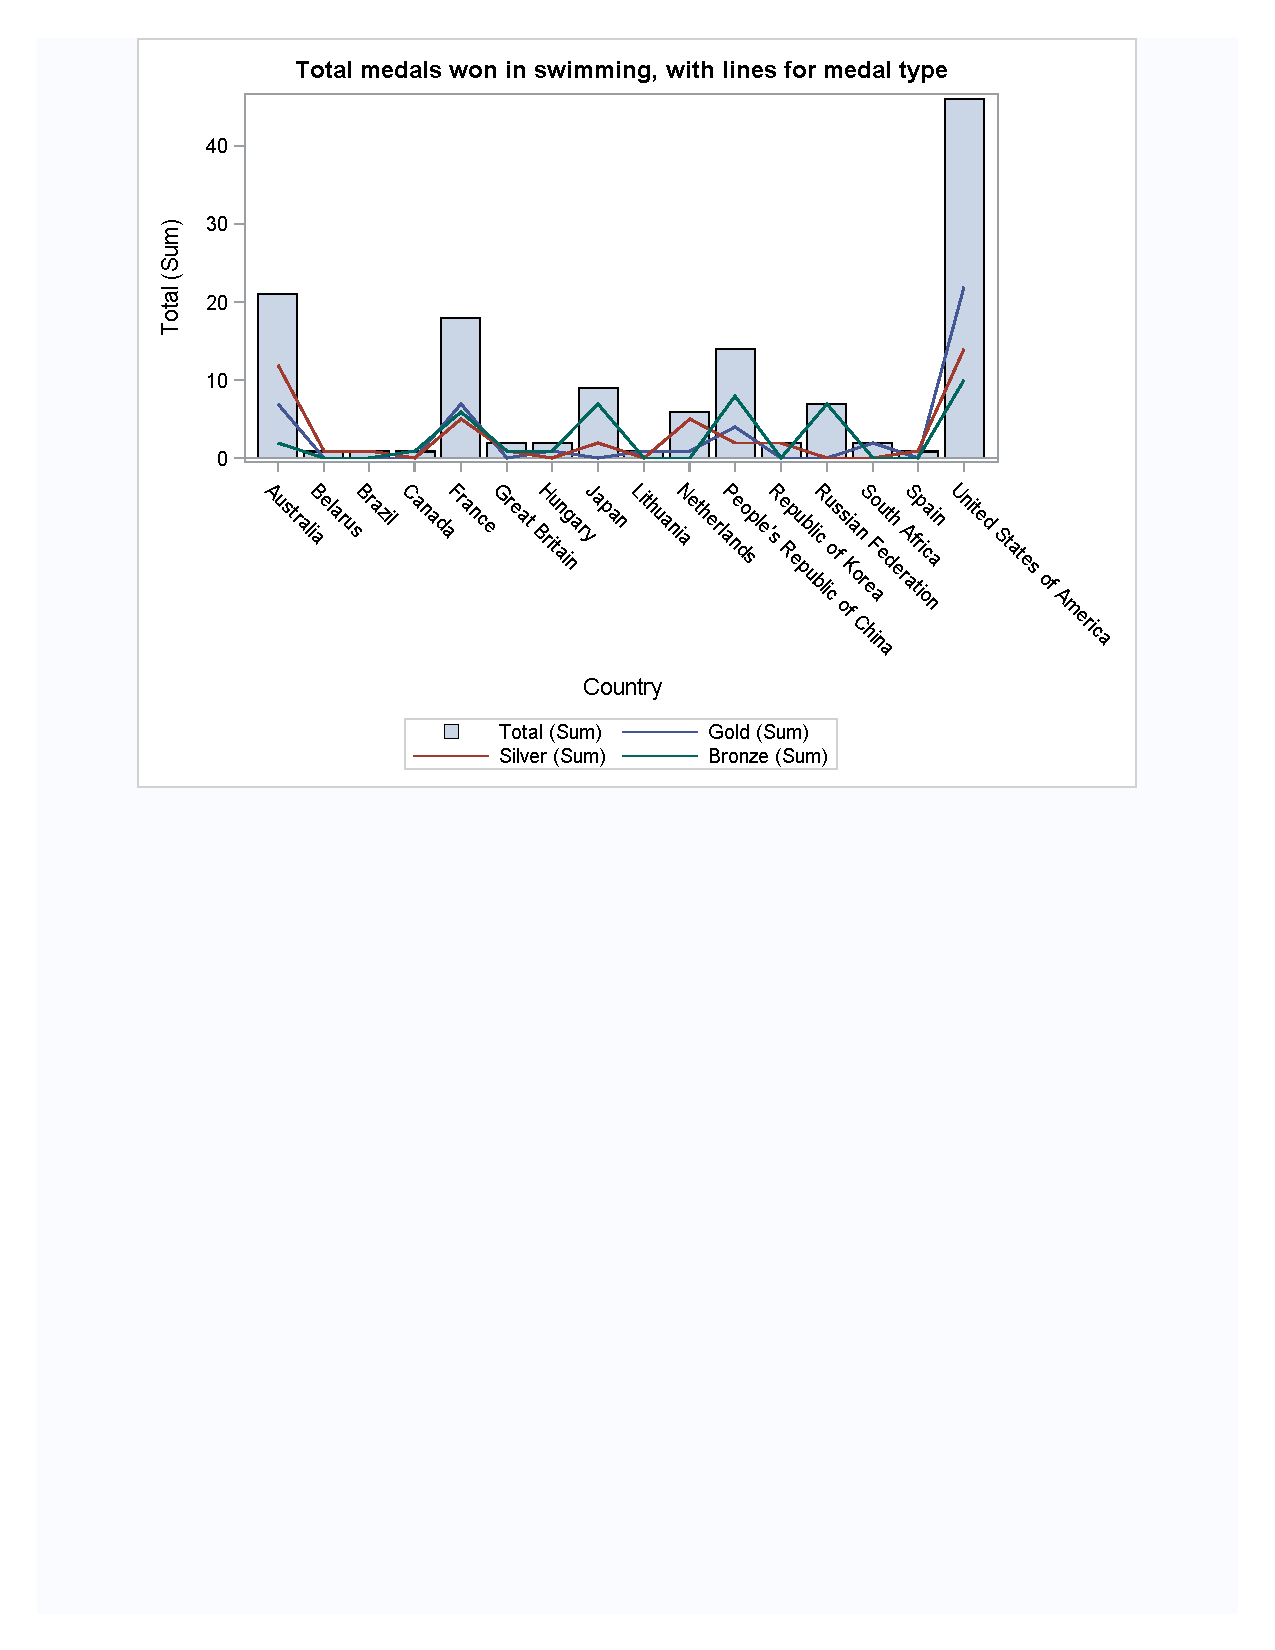
\includegraphics[trim=1.5cm 15cm 1.5cm 0cm,clip,width=1.0\textwidth]{L10_procsgplotbarplotresponselines}
\emp
\end{frame}


\begin{frame}[fragile]
\ft{Histogram with normal curve}
\bmp{1.00\textwidth}
\footnotesize
\begin{code}{.0}
PROC SGPLOT DATA = flash.o2012;
   WHERE sport = "Swimming";
   \textcolor{OrangeRed}{HISTOGRAM height ;}
   \textcolor{OrangeRed}{DENSITY height ;}
RUN;
\end{code}
\emp
\vspace{1ex}
\bmp{0.6\textwidth}
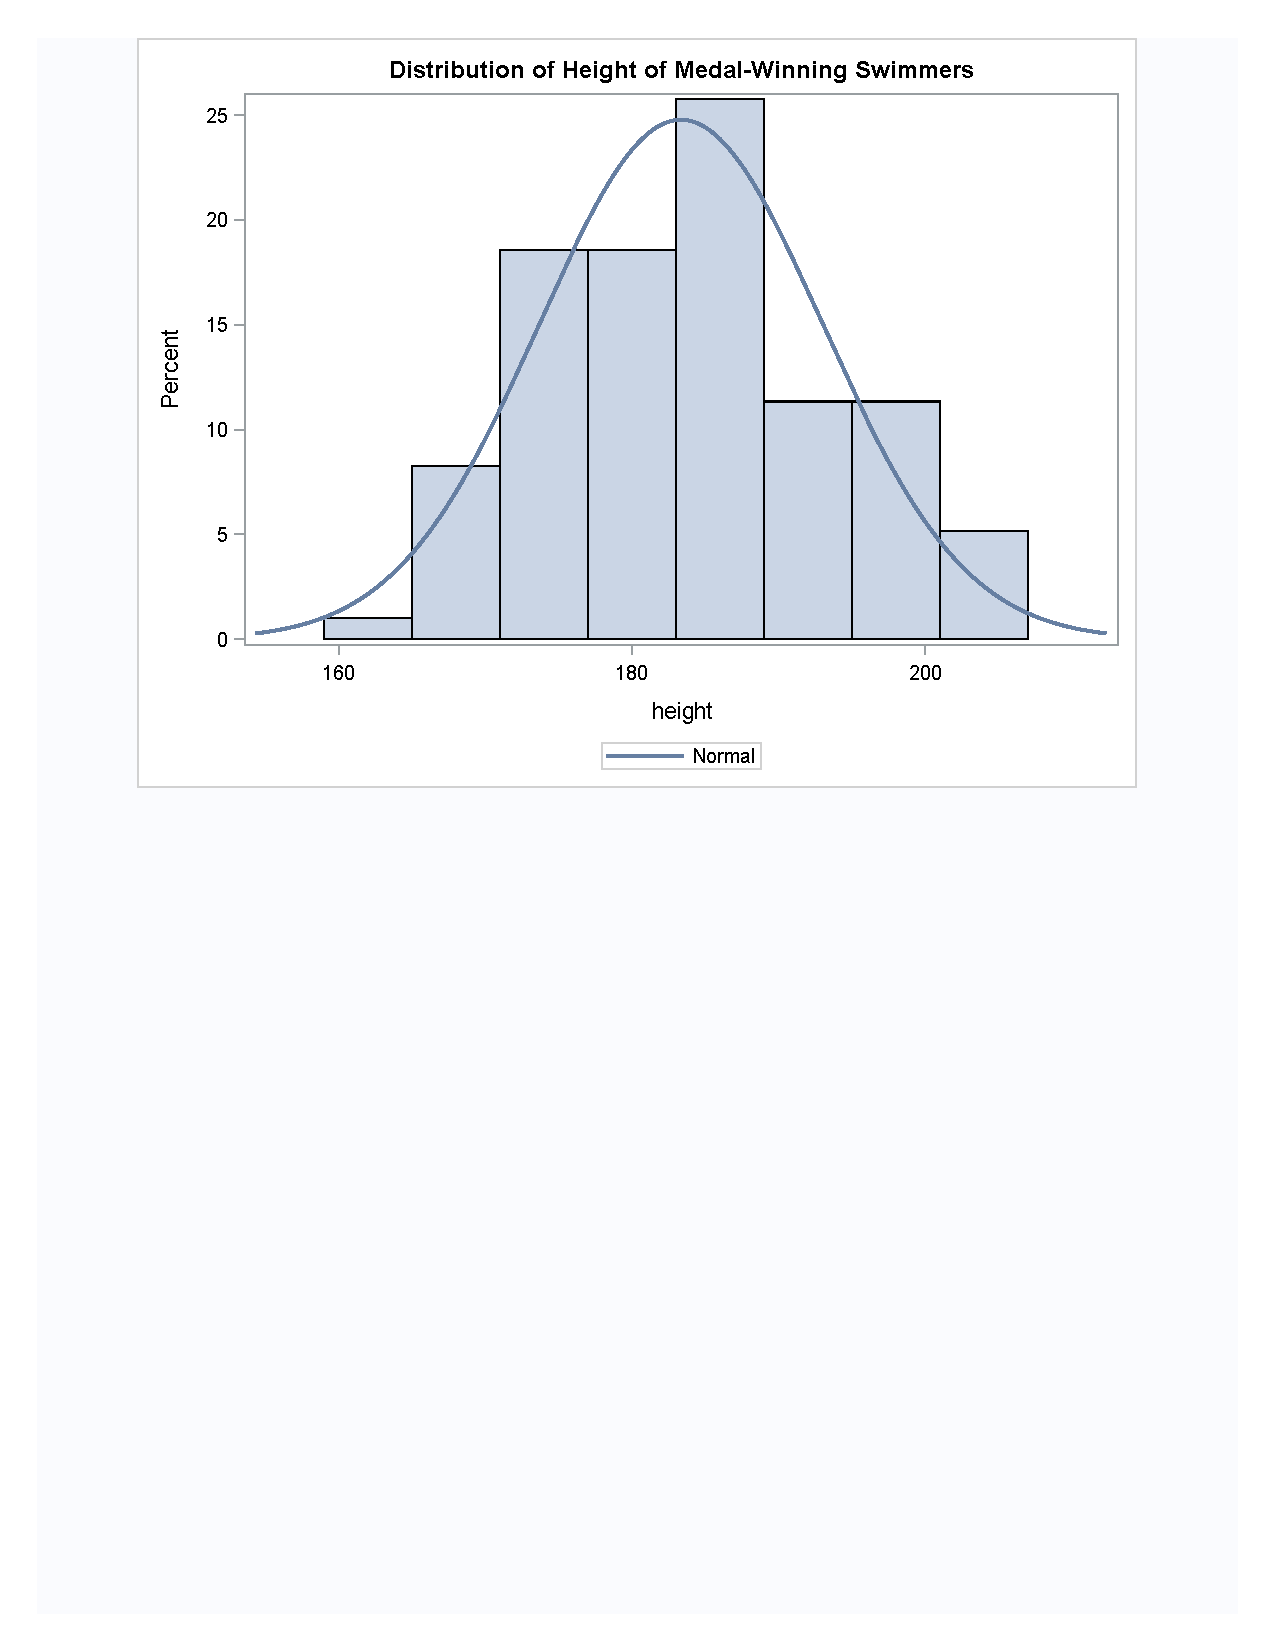
\includegraphics[trim=1.5cm 15cm 1.5cm 0cm,clip,width=1.0\textwidth]{L10_histnormal}
\emp
\end{frame}

\begin{frame}[fragile]
\ft{Histogram, density overlayed}
\bmp{1.00\textwidth}
\footnotesize
\begin{code}{.0}
PROC SGPLOT DATA = flash.o2012;
   WHERE sport="Swimming" OR sport="Gymnastics - Artistic";
   HISTOGRAM height/  \textcolor{OrangeRed}{GROUP = sport TRANSPARENCY = 0.5};
RUN ;
\end{code}
\emp
\vspace{1ex}
\bmp{0.6\textwidth}
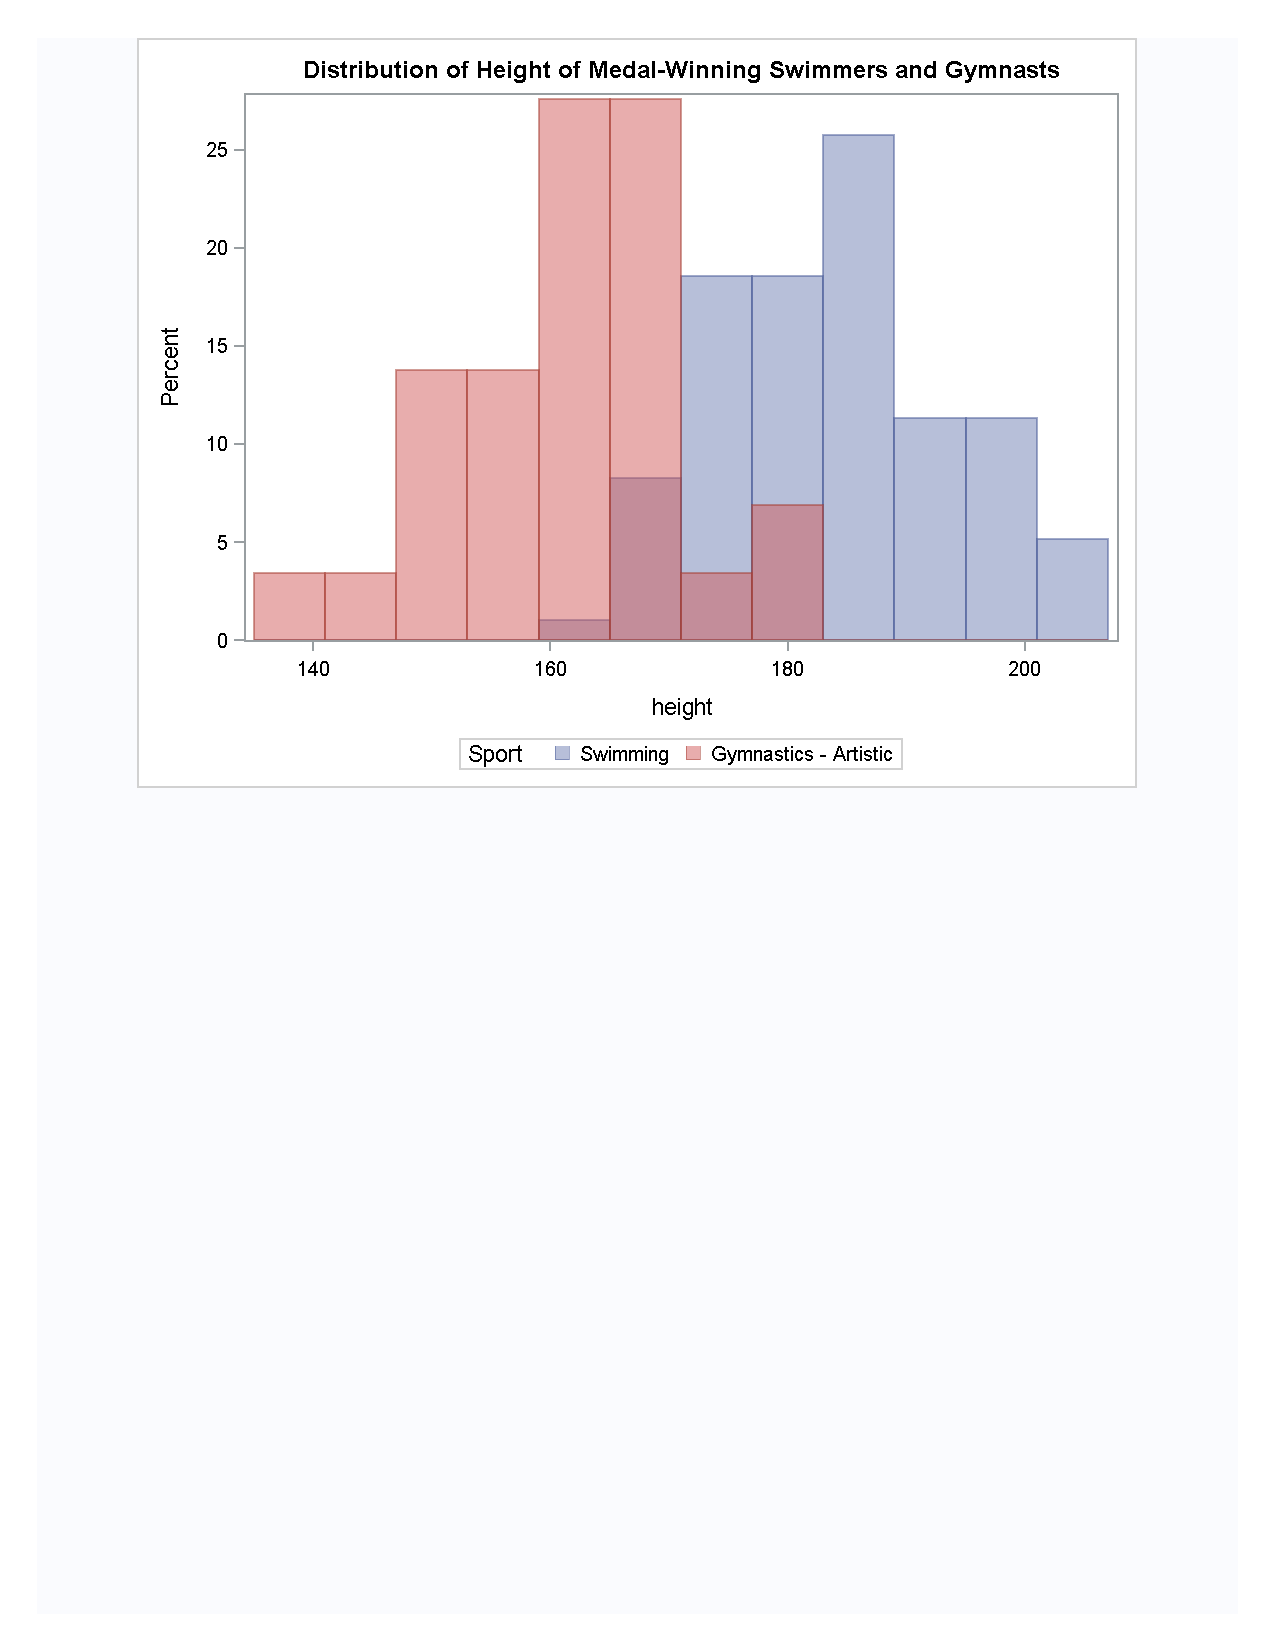
\includegraphics[trim=1.5cm 15cm 1.5cm 0cm,clip,width=1.0\textwidth]{L10_histnormaloverlay}
\emp
\end{frame}

\begin{frame}
\ft{Discussion}
\begin{clicker}{To create overlaid histograms that shows the distribution of height and weight, you need \underline{(1/2/3)}; to create overlaid histograms that shows how the distribution of height among males and females you need \underline{(1/2/3)}.}
\begin{enumerate}
\item two \ttt{HISTOGRAM} statements
\item 1 \ttt{HISTOGRAM} statement with \ttt{GROUP} option
\item either
\end{enumerate}
\end{clicker}
\end{frame}

\begin{frame}[fragile]
\ft{Side by Side Boxplot, with CATEGORY option}
\bmp{1.00\textwidth}
\footnotesize
\begin{code}{.0}
PROC SGPLOT DATA = flash.o2012;
   HBOX height / CATEGORY = sport ;
RUN ;
\end{code}
\emp
\vspace{1ex}
\bmp{0.6\textwidth}
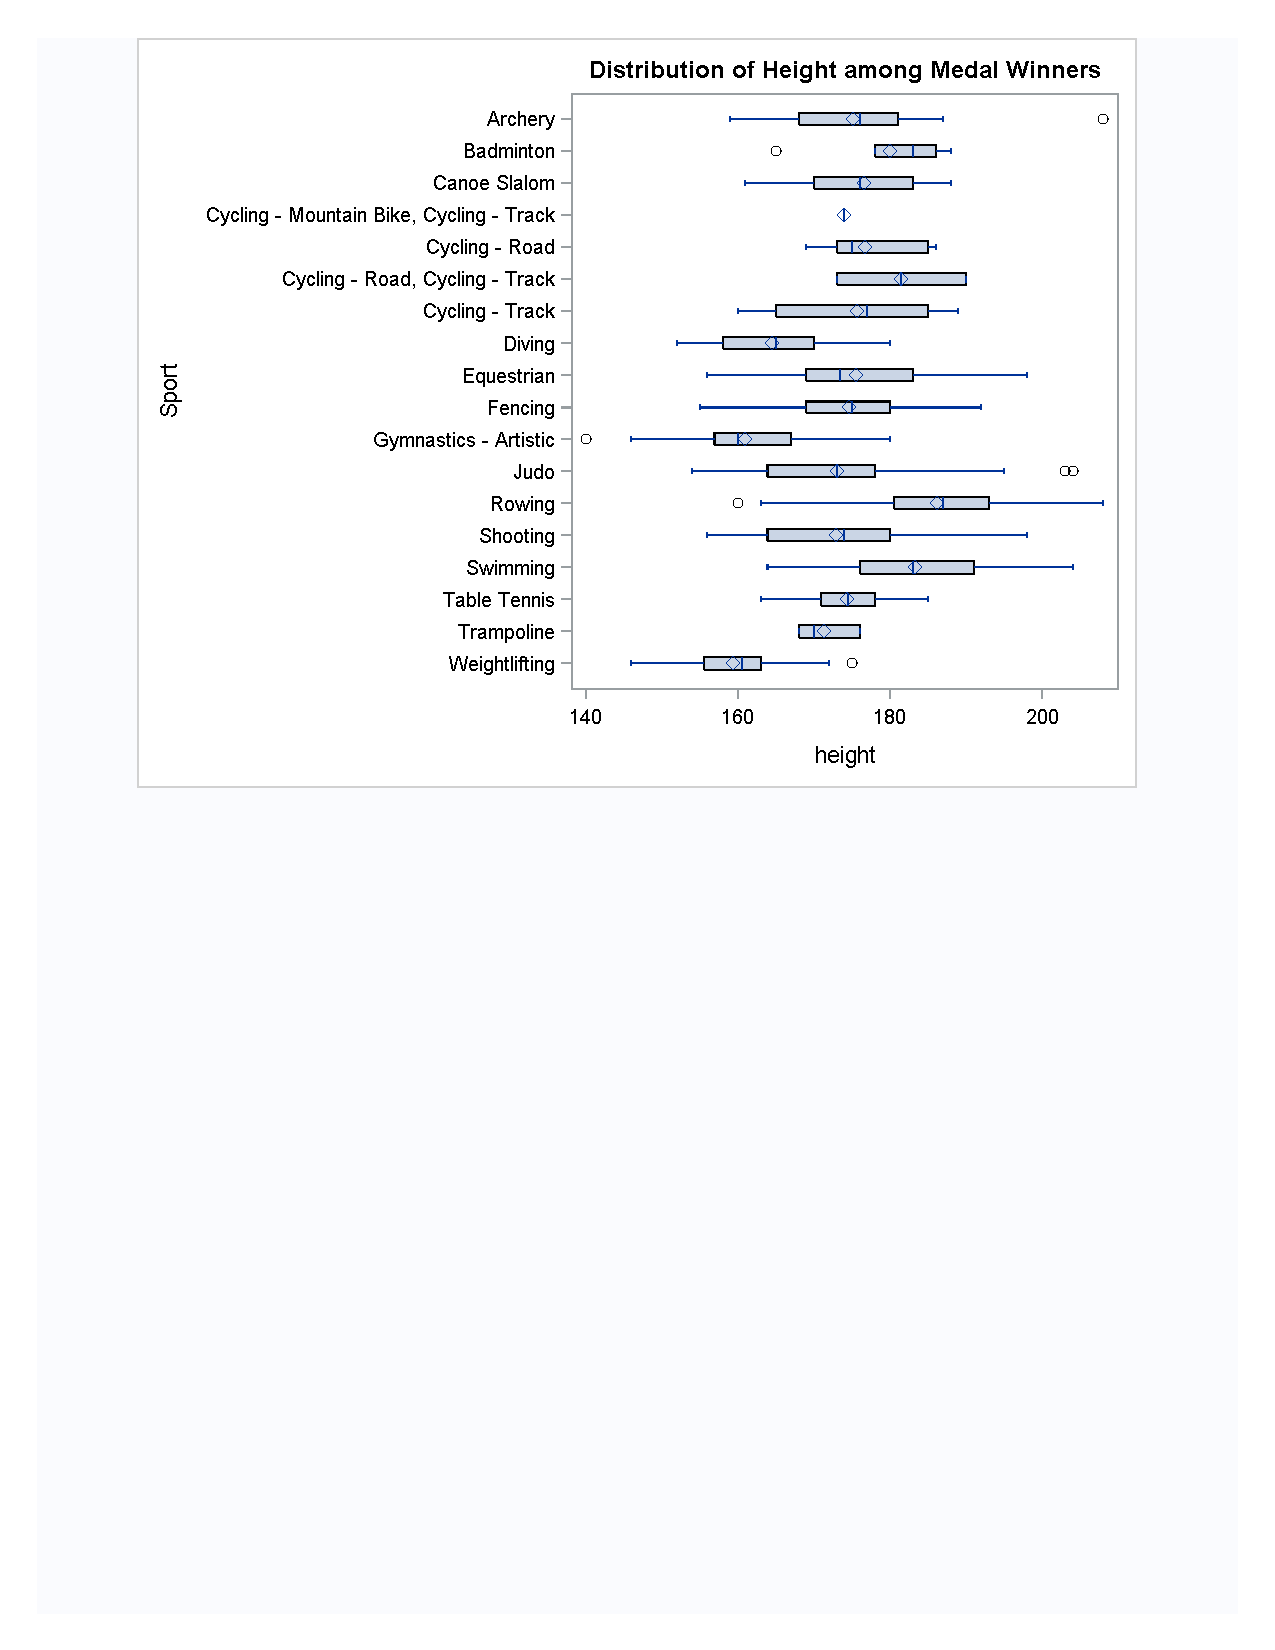
\includegraphics[trim=1.5cm 15cm 1.5cm 0cm,clip,width=1.0\textwidth]{L10_sideboxcategory.pdf}
\emp
\end{frame}


\begin{frame}[fragile]
\ft{Scatterplot}
\bmp{1.00\textwidth}
\footnotesize
\begin{code}{.0}
PROC SGPLOT DATA = flash.o2012 ;
   SCATTER Y = weight X = height ;
   XAXIS LABEL = "Height" ;
   YAXIS LABEL = "Weight" ;
   REG Y = weight X = height / CLM CLI ;
RUN ;
\end{code}
\emp
\vspace{1ex}
\bmp{0.5\textwidth}
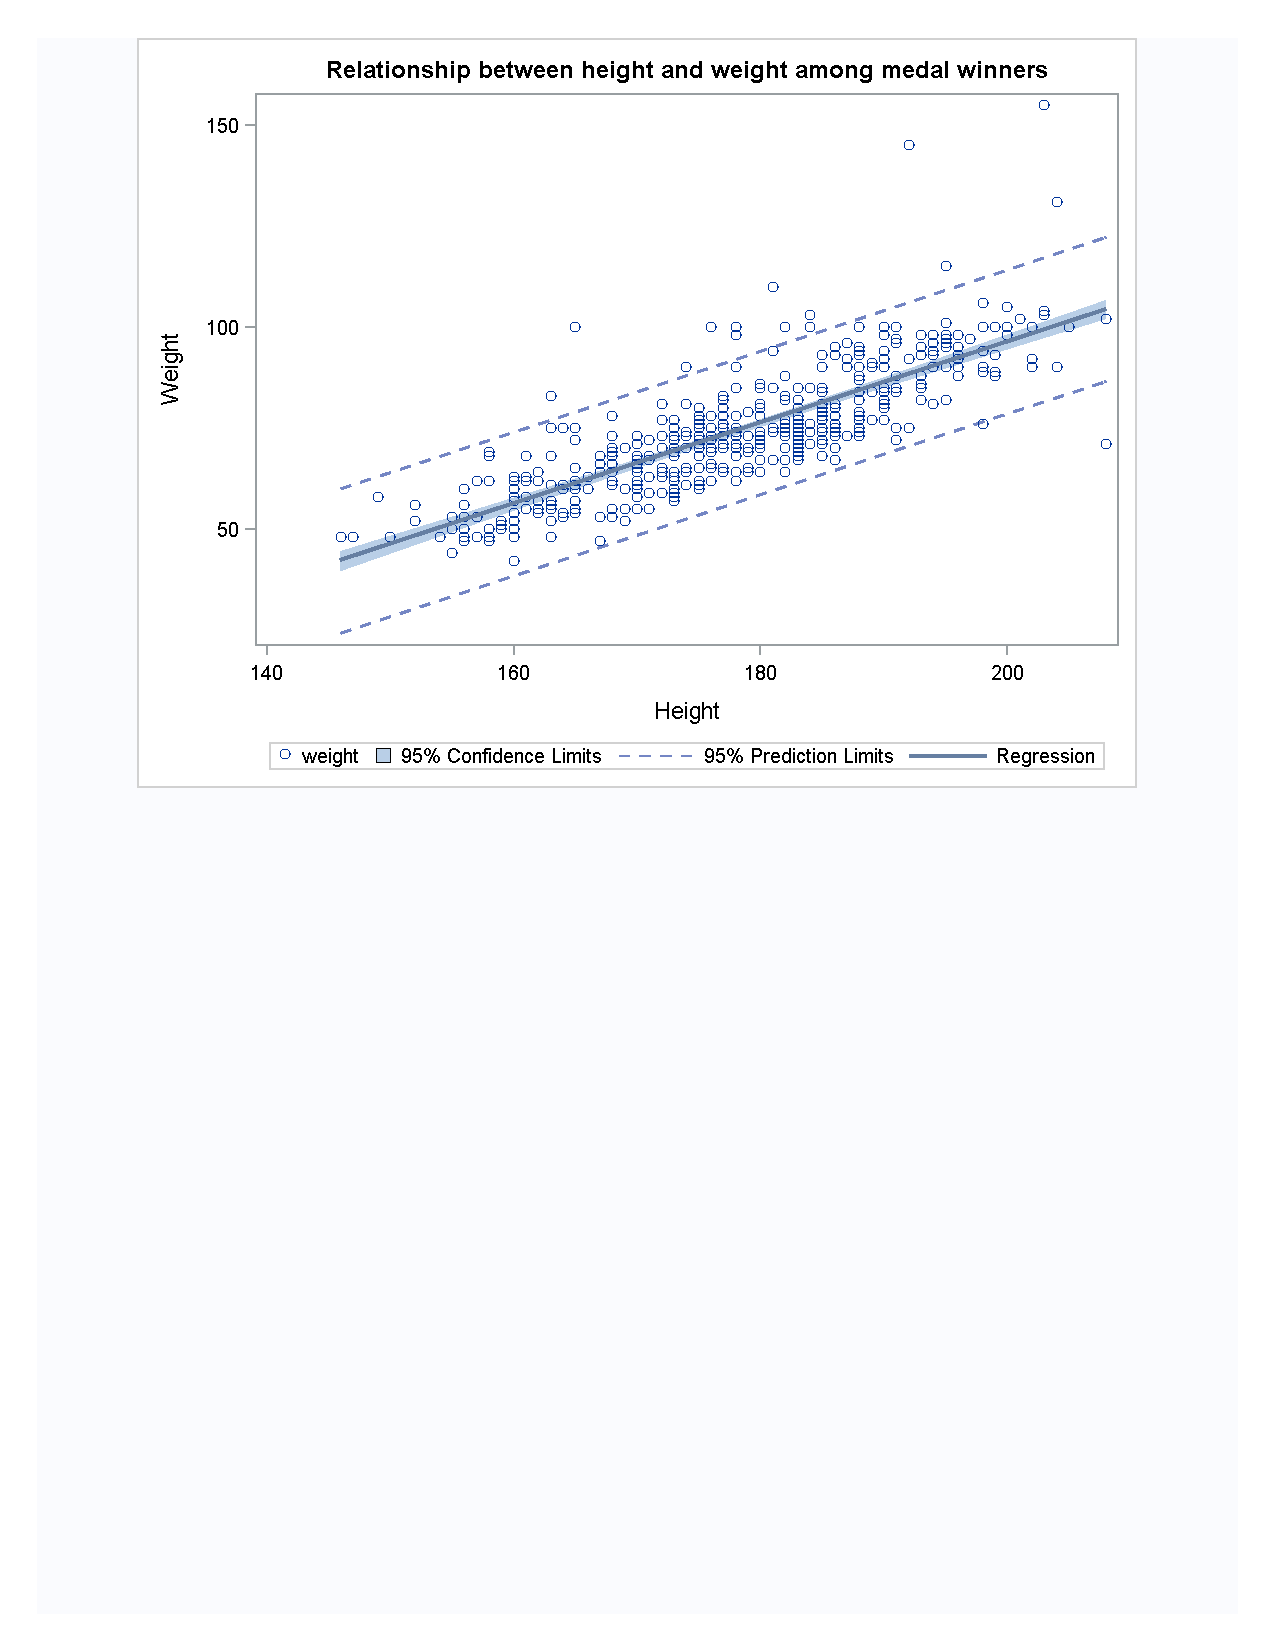
\includegraphics[trim=0.5cm 15cm 1.5cm 0cm,clip,width=1.0\textwidth]{L10_scatter1.pdf}
\emp
\end{frame}


\begin{frame}[fragile]
\ft{Scatterplot, points colored by categorical variable}
\bmp{1.00\textwidth}
\footnotesize
\begin{code}{.0}
PROC SGPLOT DATA = flash.o2012 ;
   WHERE sport = "Swimming" or sport = "Rowing" ;
   SCATTER Y = weight X = height /
      GROUP = sport
      MARKERATTRS = (symbol = CircleFilled) ;
RUN ;
\end{code}
\emp
\vspace{1ex}
\bmp{0.5\textwidth}
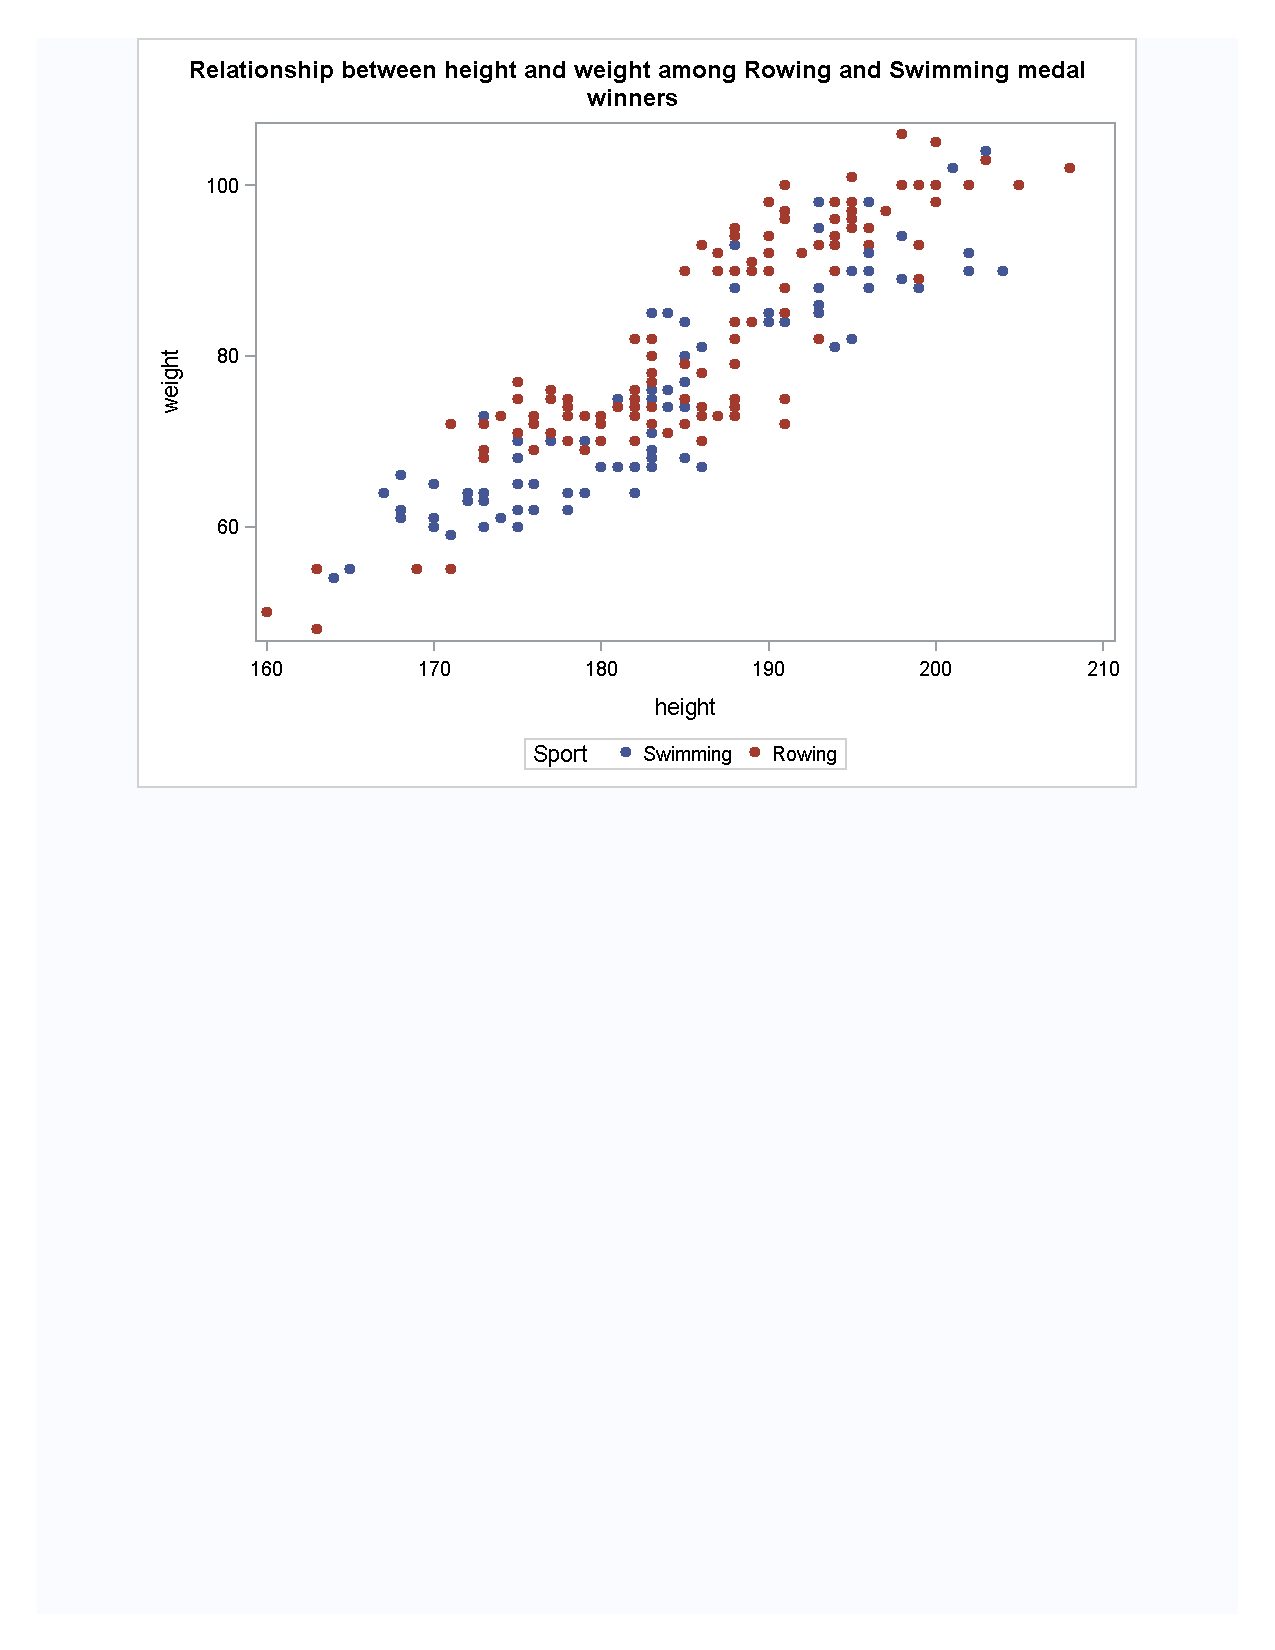
\includegraphics[trim=0.5cm 15cm 1.5cm 0cm,clip,width=1.0\textwidth]{L10_scatter2.pdf}
\emp
\end{frame}


\begin{frame}[fragile]
\ft{Scatterplot, points colored by quantitative variable}
\bmp{1.00\textwidth}
\footnotesize
\begin{code}{.0}
PROC SGPLOT DATA = flash.o2012 ;
   SCATTER Y = weight X = height /
     COLORRESPONSE = age
     MARKERATTRS = (symbol=CircleFilled size=10)
     COLORMODEL = TwoColorRamp;
RUN ;
\end{code}
\emp
\vspace{1ex}
\bmp{0.5\textwidth}
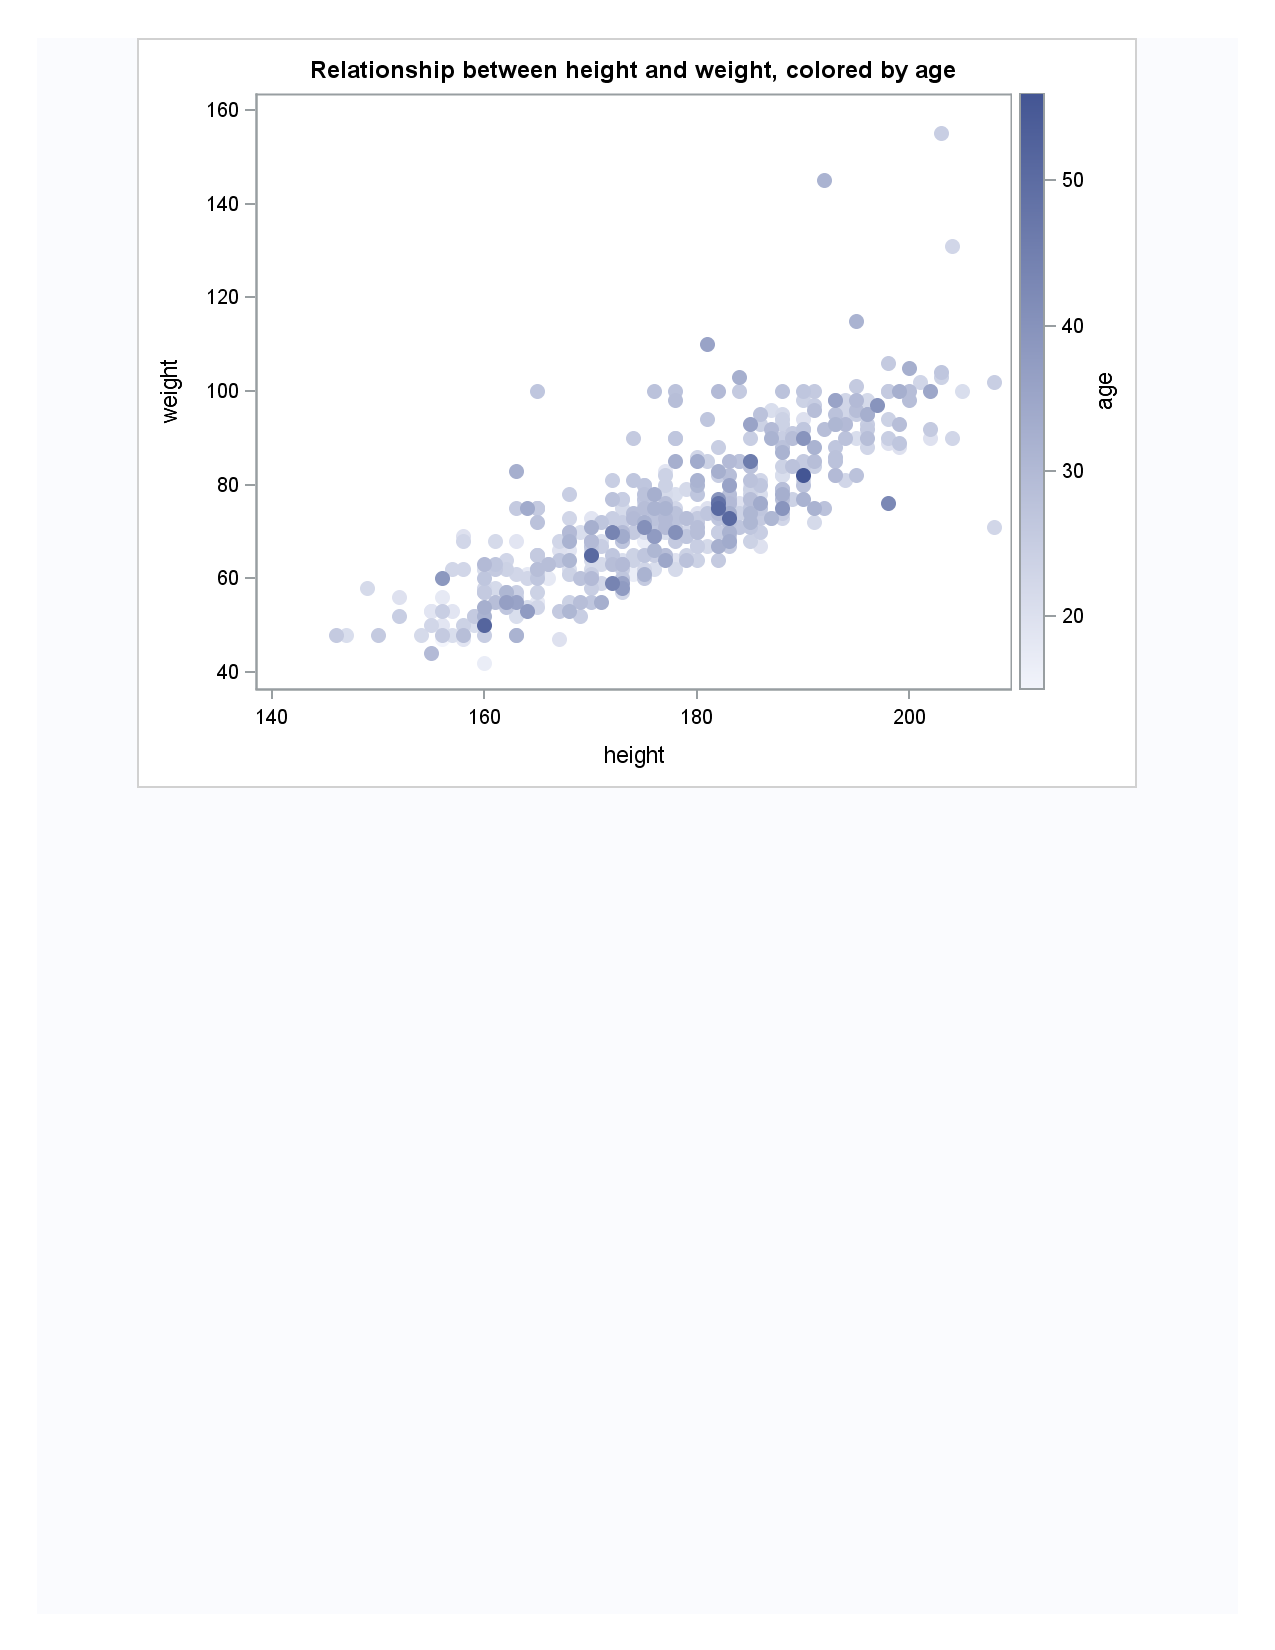
\includegraphics[trim=0.5cm 15cm 1.5cm 0cm,clip,width=1.0\textwidth]{L10_scatter3.pdf}
\emp
\end{frame}



\begin{frame}[fragile]
\ft{Group vs  Category Option}
\bi
\item In general, both \ttt{GROUP} and \ttt{CATEGORY} options can be used in the SGPLOT statements (ie, HBAR, SCATTER, etc).
\item The output does look different with the two options.
\item The \ttt{group} option results in graphical elements that have varying attributes
\bi
\item Each unique value of the grouping variable is drawn in a separate style element GraphData$1$ through GraphData$k$
\item Produces a legend matching graphical styles to group
\ei
\item If you want \textbf{different colors} - try \ttt{GROUP}
\item If you want \textbf{same color} and a legend - try \ttt{CATEGORY}
\item More info: \url{https://blogs.sas.com/content/iml/2012/08/22/categories-vs-groups-in-proc-sgplot.html}
%\bi
%\item \ttt{HBAR/VBAR} uses \ttt{group}
%\item \ttt{HISTOGRAM} uses \ttt{group}
%\item \ttt{VBOX/HBOX} uses \ttt{category}
%\item \ttt{SCATTER}   uses \ttt{group}
%\item \ttt{SERIES}    uses \ttt{group}
\ei

\end{frame}


\end{document} 